
\subsection{Input parameters}
\label{sec:input}


In PyECLOUD, photoelectrons are generated simultaneously with the beam charge.
Figure~\ref{fig:input} shows the related input parameters of the code, these are explained in more details in the following pages.
%It can be specified how many electrons per proton are generated and how they are distributed around the 2D chamber walls.

\begin{figure}[tbh]
    \centering
    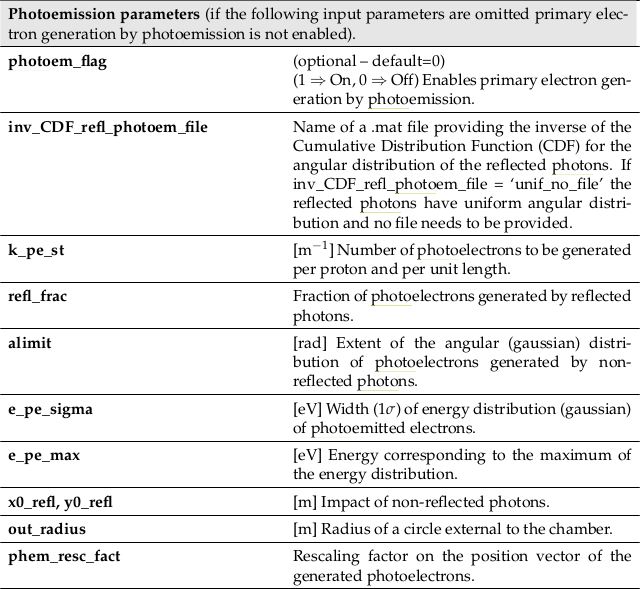
\includegraphics[width=0.8\textwidth]{../ss/pyecloud_doc.png}
    \caption{The input parameters of the PyECLOUD simulation code regarding photoemission seeding.}
    \label{fig:input}
\end{figure}

The quantity \textbf{k\_pe\_st} is the total number of photoelectrons per proton and m.
\\
The quantity \textbf{refl\_frac} is the ratio between all photoelectrons and those that origin from reflected photons.

The generation of photoelectrons created by immediately absorbed photons and reflected photons differs in PyECLOUD, see Fig.~\ref{fig:gt}.
For both of them, an angle relative to the center of the chamber is randomly generated.
In the case of non-reflected photons, this angle is Gaussian distributed with a standard deviation of \textbf{a\_limit}.
In the case of reflected photons, an angle of reflection with respect to the impact point is obtained from a given distribution.
The point where photoelectrons are generated is determined as the intersection of the line between a point on the outer circle  and the origin with a chamber wall.

\textbf{inv\_CDF\_refl\_photoem\_file} includes the inverse cumulative distribution function (CDF) for the angles under which the photons are reflected from the impact point.

Photoelectrons are emitted with a truncated Gaussian energy distribution, specified by \textbf{e\_pe\_sigma} and \textbf{e\_pe\_max} with only positive energies allowed.
Their initial direction is found through a cosine distribution for the angle with respect to the surface normal at these points.
\begin{figure}[tbh]
    \centering
    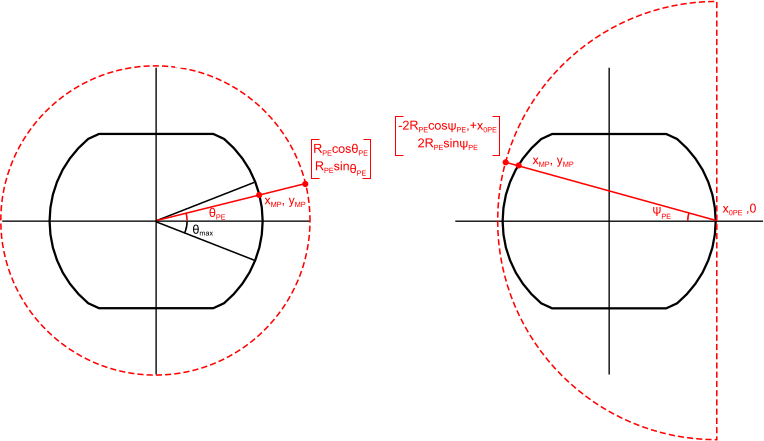
\includegraphics[width=0.8\textwidth]{../ss/gianni_thesis_photoelectrons.png}
    \caption{Position generation algorithm for photoelectrons from non-reflected (left) and reflected (right) photons~\cite{gianni}.}
    \label{fig:gt}
\end{figure}


\textbf{out\_radius} describes a circle that encloses the beam chamber, see Fig.~\ref{fig:gt}.

\textbf{x\_0\_refl} and \textbf{y\_0\_refl} are coordinates that have to be located inside the chamber.
This point together with an angle of reflectivity leads to the positions of new MPs from reflected photons, see Fig.~\ref{fig:gt}.
Cases where y\_0\_refl is nonzero are not yet supported.

\subsection{Validation}

A script to generate the plots shown in Fig.~\ref{fig:test_module} is part of the "photoemission" branch of PyECLOUD on GitHub ("test\_photoemission.py").
It calls the photoemission module to produce these plots, and verifies the expected behavior.
\begin{figure}[tbh]
    \centering
    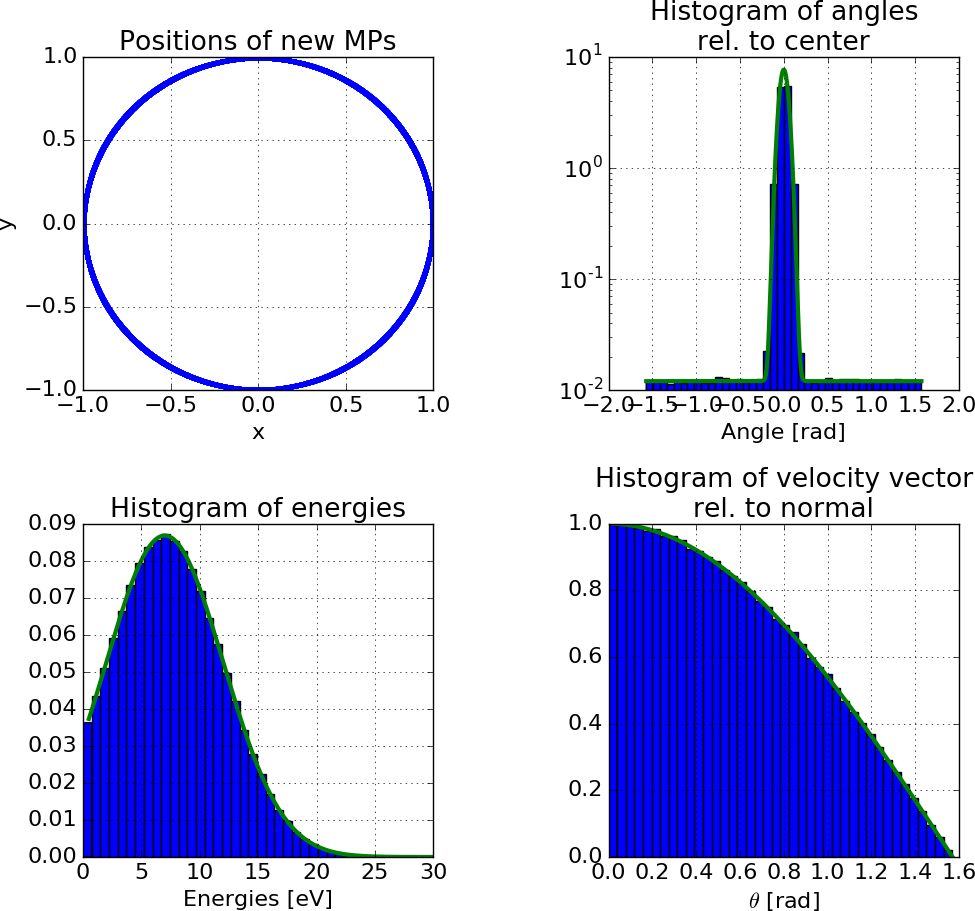
\includegraphics[width=0.8\textwidth]{../plots/test_module.png}
    \caption{
        The photoemission seeding is validated with these tests.
        The top two plots show the positions of new macroparticles for a circular chamber.
        The green line is the expected behavior for an alimit of 0.05 and a refl\_frac of 3.8\%, given a uniform distribution of reflected photons.
        The bottom plots show the energies and angles relative to the impact normal for new macroparticles.
    }
    \label{fig:test_module}
\end{figure}

